\documentclass[addpoints, 11pt,a4paper]{exam}
\usepackage{graphicx}
\usepackage{float}
\usepackage[european, straightlabels]{circuitikz}
\title{Lower Shell Electricity Test}
\author{}
\date{}

\setlength\dottedlinefillheight{1cm}
\pointname{}
\newcommand{\ans}[1]{\fillwithdottedlines{#1cm} \droppoints}

\begin{document}
\pagestyle{empty}
\maketitle \thispagestyle{empty}
\begin{center}
    \makebox[0.7\textwidth]{Name:\enspace\hrulefill}
\end{center}
\pointsdroppedatright
\begin{questions}
    \question[3] A rechargeable cell draws a current of 0.1A for 10 hours. What is the total charge delivered in that time? \fillwithdottedlines{2cm} \droppoints
    \question[3] If a charge of 20 millicoulombs is delivered in 80 microseconds, what is the average current? \ans{2}
    \question[3] How many electrons would need to flow between two points each second in order to produce a current of 2 amps? (NB: The charge on an electron is  1.6 x 10$^{-19}$ coulombs.) \ans{2}
    \question A diode is an electrical component.
\begin{parts}
    \part[1] Draw the circuit symbol for a diode. \vspace{3cm} \droppoints
    \part[1] What function does it perform? \ans{2}
\end{parts}
\question[3] What is the pd across a resistor if 20J of energy is transferred when 5C of charge passes through it? \ans{2}
\question[3] How much energy is transferred when 2.5C of charge passes through a pd of 40V? \ans{2}
\question[3] What is the resistance of a component that draws a current of 1.5 A when a voltage of 9V is applied across it? \ans{2}
\question 
\begin{parts}
    \part[3] A 3kΩ resistor and a 500Ω resistor are placed in series. What current will flow if they are connected to a 14V power supply? \ans{2}
    \part[2] What will be the pd across the 500Ω resistor? \ans{2}
\end{parts}
\newpage
\question[3] Below is shown the current-voltage graph for a lightbulb.  

\begin{figure}[H]
    \centering
    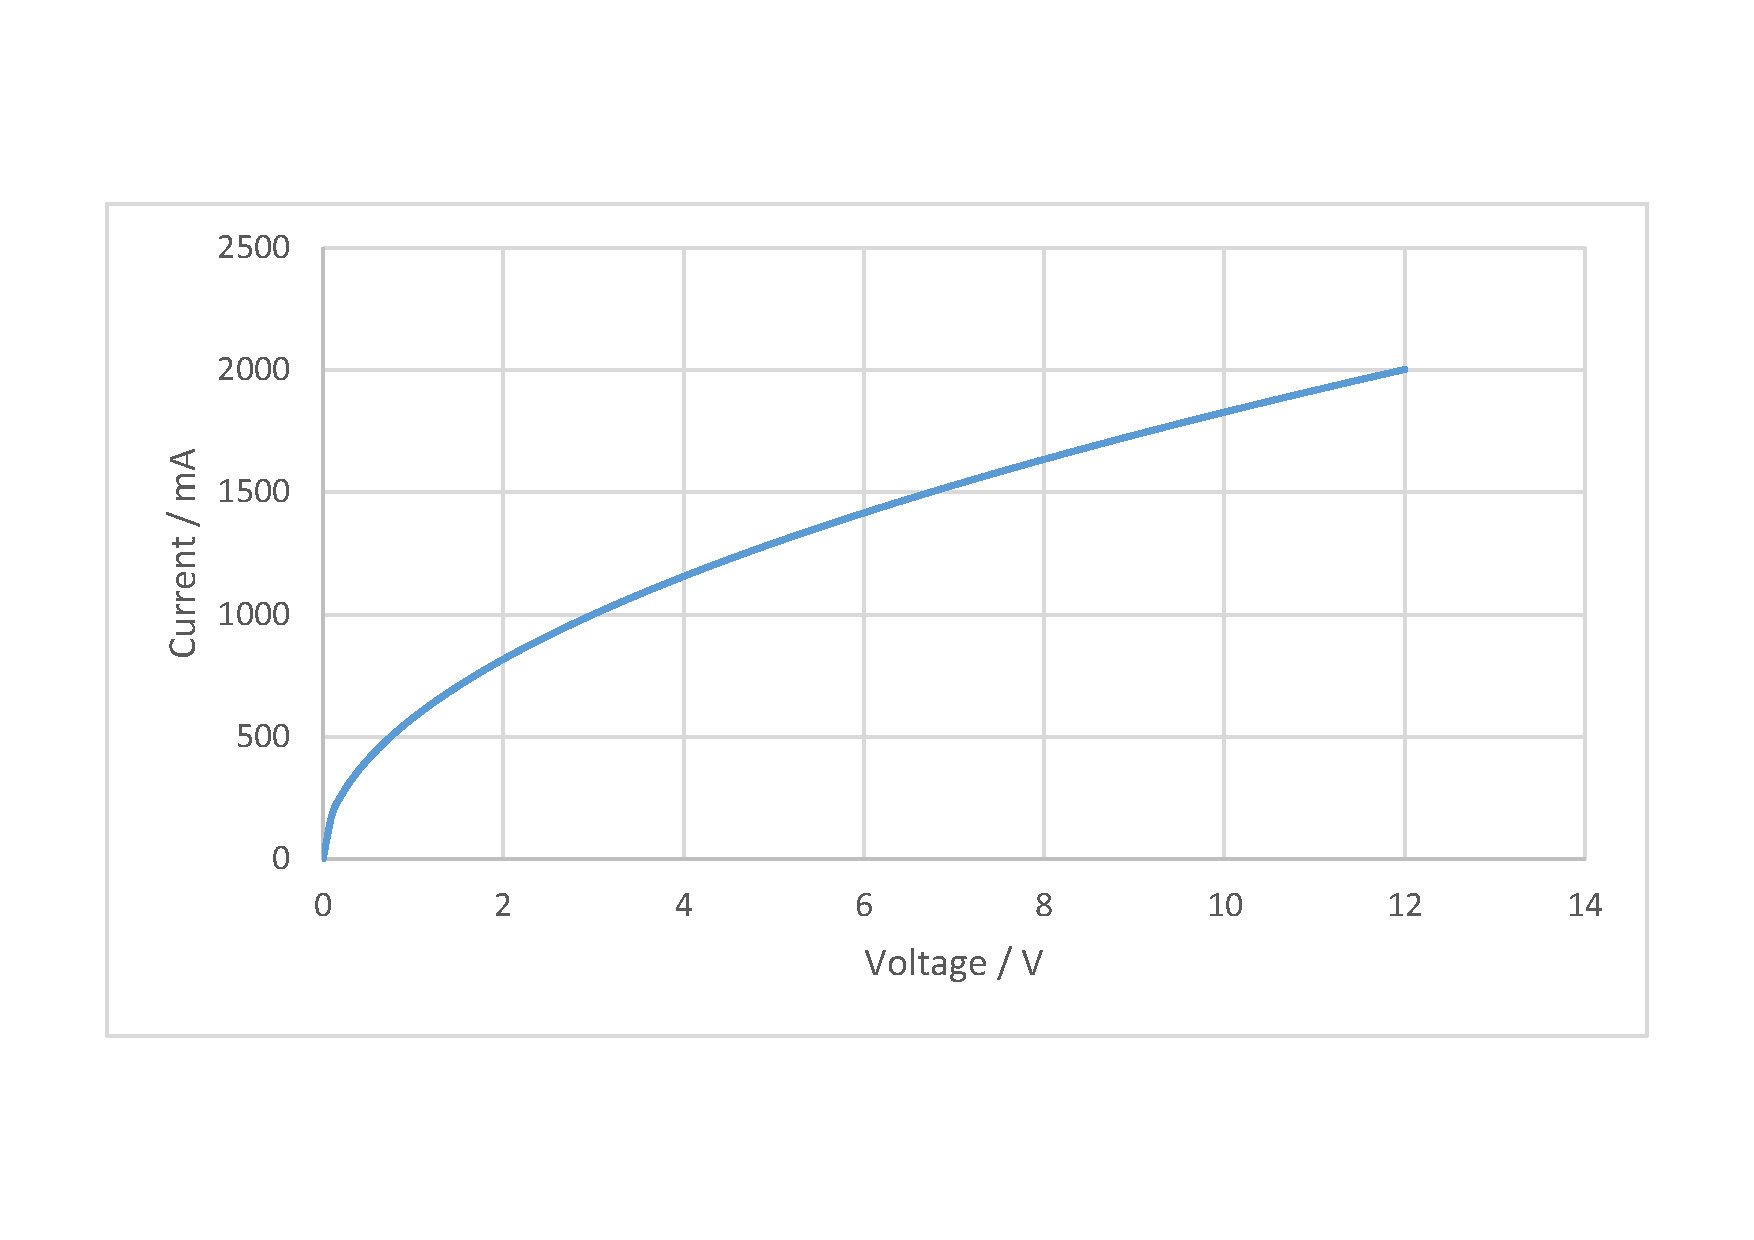
\includegraphics[width=0.8\textwidth]{img/lightbulb.pdf}
\end{figure}

Describe and explain the shape of this graph. \ans{4}

\question A  circuit is made consisting of a 10V battery, a thermistor and a 1 kΩ resistor connected in series.
\begin{parts}
    \part[3] Draw this circuit. \vspace{4cm} \droppoints
    \newpage
    \part[3] On a cold day the resistance of the thermistor is 700Ω. Calculate the voltage across the RESISTOR. \ans{3}
    \part[2] Would the voltage across the resistor be higher or lower on a warm day?  Explain your answer. \ans{3}
\end{parts}

\question[4] In the following circuit, calculate the current $I$ through the ammeter and the potential difference $V$ across the voltmeter.
\begin{figure}[H]
    \centering
\begin{circuitikz} \draw
    (0,1) to[ammeter] (0,4) 
    to[battery, l=12V] (7,4)
    -- (7,1) -- (6,1) -- (6,2) to[R, l=$20\Omega$] (4,2)  -- (4,1) to[R, l=$30\Omega$] (0,1)
    (6,1) -- (6,0) to[R, l=$24\Omega$] (4,0) -- (4,1)
    (1,1) -- (1,-.5) to[voltmeter] (3,-.5) -- (3,1);

\end{circuitikz}
\end{figure} \ans{4}
\end{questions}

\flushright{\textbf{Total Marks: \numpoints}}
\end{document}
